\documentclass[a4paper, 10pt]{article}

% Use packages here
\usepackage[a4paper, left=1cm, right=1cm, top=1.5cm, bottom=2cm]{geometry}
\usepackage{blindtext} % This package is used for testing
\usepackage[british]{babel} % This package is used for localisation
\usepackage{paralist} % This package creates compact lists
\usepackage{multicol} % This package arranges contents in columns
\usepackage{indentfirst} % This package is used for indentation in paragraphs
\usepackage{array}
\usepackage{amsmath} % This package is used for conditional math equations
\usepackage{graphicx} % This package is used for inserting and manipulating on images
\usepackage{titlesec} % For section, subsection and subsubsection and so on.
\usepackage{caption}
\newenvironment{Figure}
    {\par\medskip\noindent\minipage{\linewidth}}
    {\endminipage\par\medskip}

% Preamble here
\setlength\columnsep{20pt} % This is the default columnsep for all pages

\setcounter{secnumdepth}{4}

\graphicspath{ {../Diagrams/} {../Diagrams/KeyExpansion/} }

\hyphenation{
    trans-form-ation 
    exponent-ially 
    crypto-graphic
    crypto-graphy 
    sub-titu-tion 
    ta-ble 
    rou-tine 
    rectang-ular 
    expan-sion 
    secur-ity 
    encryp-tion 
    decryp-tion 
    specifi-cation 
    inter-mediate 
    multi-pli-cation 
    poly-nomials 
    compris-ing 
    stand-ard
}

% Document begins here
\begin{document}

    %%%%%%%%%
    % TITLE %
    %%%%%%%%%
    \title{\centering{IMPLEMENTING AES-256 ON FPGA}}
    \author{}
    \maketitle % Call this command to make title

    \begin{center}
        Ho Hai Cong Thuan\\
        Student, Computer Engineering, University of Information Technology, HCMC, Vietnam\\
        hohaicongthuan@gmail.com
    \end{center}
    \begin{multicols}{2}
        
        %%%%%%%%%%%%
        % ABSTRACT %
        %%%%%%%%%%%%
        \textbf{\textit{Abstract\textemdash}In the modern days, the amount of data grow exponentially, including classified and sensitive data that need to be kept secured. For this reason, many cryptographic techniques have been invented for the purpose. AES is one of them. It provides fast and secure data encryption which are the reasons this algorithm is chosen for this project.}

        \textbf{The goal of this project is to implement a fully functional AES encryption and decryption system using 256-bit key on FPGA.}
        
        \bigskip

        \textbf{\textit{Keywords\textemdash}AES-256; cryptography; data security; FPGA; encryption; decryption.}

        %%%%%%%%%%%
        % CONTENT %
        %%%%%%%%%%%
        \section{INTRODUCTION}
            \textit{The Advanced Encryption Standard (AES)}, also known as \textit{Rijndael} is a specification for encrypting electronic data first introduced by the \textit{U.S. National Institute of Standards and Technology (NIST)} in 2001. It provides a fast and secure way to encrypt data and uses symmetric keys encryption which means both the encryption and decryption processes using the same key. The key length for AES could be 128, 192 and 256 bits. This paper concentrates on AES using 256-bit key which will be refered to as AES-256 for the rest of this paper.
            
            \subsection{Concepts used in AES-256}
                % \begingroup
                    % \setlength{\tabcolsep}{10pt} % Default value: 6pt
                    % \renewcommand{\arraystretch}{1.5} % Default value: 1
                    \noindent
                    \begin{tabular}{m{2cm} m{5cm}}
                        \textbf{\textit{Key expansion}} & Routine used to generate a series of Round Keys from the Cipher Key.\\
                        \hline
                        \textbf{\textit{State}} & Intermediate Cipher result that can be pictured as a rectangular array
                        of bytes, having four rows and \textbf{\textit{Nb}} columns.\\
                        \hline
                        \textbf{\textit{S-box}} & Non-linear substitution table used in several byte substitution transformation and in the Key Expansion routine to perform a one-for-one substitution of a byte value.\\
                        \hline
                        \textbf{\textit{Word}} & A group of 32 bits that is treated either as a single entity or as an array of 4 bytes.\\
                    \end{tabular}
                % \endgroup
            
            \subsection{Abbreviations and Symbols used in AES-256}
                % \begingroup
                    \setlength{\tabcolsep}{5pt} % Default value: 6pt
                    \renewcommand{\arraystretch}{1.5} % Default value: 1
                    \noindent
                        \begin{tabular}{m{1cm} m{6.5cm}}
                            \textbf{\textit{Nb}} & Number of columns (32-bit words) comprising the State. For this
                            standard, \textbf{\textit{Nb}} = 4.\\
                            \hline
                            \textbf{\textit{Nk}} & Number of 32-bit words comprising the Cipher Key. For this standard, \textbf{\textit{Nk}} = 8.\\
                            \hline
                            \textbf{\textit{Nr}} & Number of rounds, which is a function of \textbf{\textit{Nk}} and \textbf{\textit{Nb}} (which is
                            fixed). For this standard, \textbf{\textit{Nr}} = 14.\\
                            \hline
                            XOR & Exclusive-OR operation\\
                            \hline
                            $\oplus$ & Exclusive-OR operation\\
                            \hline
                            $\otimes$ & Multiplication of two polynomials (each with degree $<$ 4) modulo $x^{4}+1$\\
                            \hline
                            $\bullet$ & Finite field multiplication\\
                        \end{tabular}
                % \endgroup

        \section{AES-256}
            \subsection{Key Expansion}
                The Key Expansion routine in AES-256 takes a 256-bit cipher key and generate a set of $Nb(Nr+1)$ (which is 60) words. These words are smaller parts that make up round keys, each round key has four words. These round keys involve in the \textit{Add Round Key} in the encryption and decryption process.

                There are 3 functions that participate in the key scheduling process:

                % \begingroup
                    \setlength{\tabcolsep}{5pt} % Default value: 6pt
                    \renewcommand{\arraystretch}{1.5} % Default value: 1
                    \noindent
                        \begin{tabular}{m{2cm} m{6cm}}
                            \textbf{\textit{RotWord}} & Takes a four-byte word $[a_{0},a_{1},a_{2},a_{3}]$ and performs rotation one byte to the left and returns $[a_{1},a_{2},a_{3},a_{0}]$.\\
                            \hline
                            \textbf{\textit{SubWord}} & Takes a four-byte word and substitute each byte with the corresponding byte in the S-box.\\
                            \hline
                            \textbf{\textit{Rcon}} & The round constants, which is given in the form $[rc_{i},00_{16},00_{16},00_{16}]$ with $i$ starts from 1. $rc_{i}$ is defined as in (1)\\
                        \end{tabular}
                    \end{multicols}

                    %%%%%%%%%%%%%%%%
                    % S-BOX FIGURE %
                    %%%%%%%%%%%%%%%%
                    \noindent
                    \begin{figure}[t]
                        \centering
                        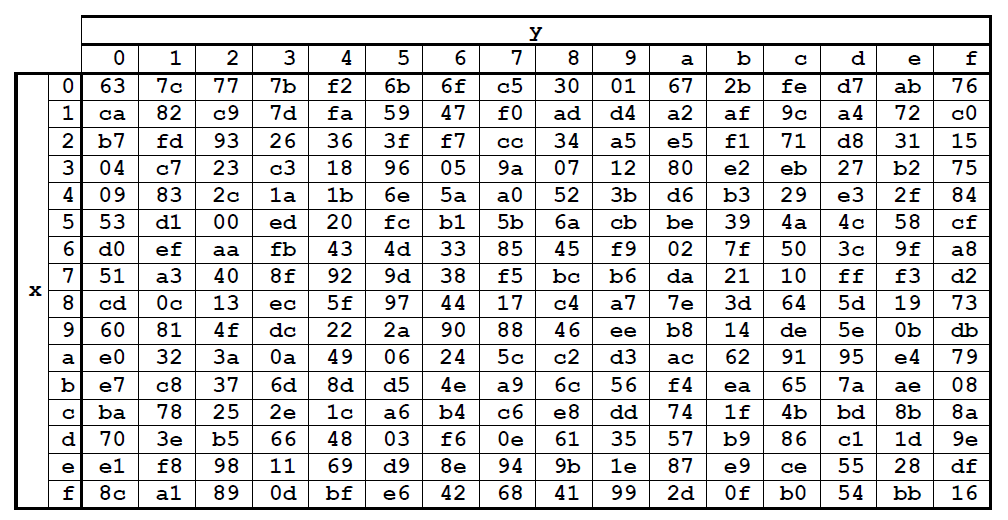
\includegraphics[width=.75\textwidth]{S-Box.png}
                        \caption{Substitution Box (S-Box) used in SubBytes transformation.}
                        \label{fig:SBox}
                    \end{figure}

                    \begin{multicols}{2}
                        \begin{equation}
                            rc_{i}=
                            \begin{cases}
                                1 & \text{if } i=1\\
                                2 \cdot  rc_{i-1} & \text{if } i>1 \text{ and } rc_{i-1}<80_{16}\\
                                \left(2 \cdot  rc_{i-1}\right)\oplus 11\text{B}_{16} & \text{if } i>1 \text{ and } rc_{i-1} \ge 80_{16}
                            \end{cases}
                        \end{equation}
                % \endgroup

            \subsubsection{Algorithm}
                In AES-256, the first two round keys (first 8 words) are filled with the cipher key. For the rest, $w[i]$ word is generated using $w[i-1]$ word.

                Loop through the following steps until we have generated $Nb(Nr+1)$ words.

                If $i$ is divisible by \textbf{\textit{Nk}}, $w[i-1]$ is rotated by the function \textbf{\textit{RotWord}} and then substituted by the function \textbf{\textit{SubWord}}. The final result is \textbf{\textit{XOR}}-ed with \textbf{\textit{Rcon[i/Nk]}} and assigned to $w[i]$. Otherwise, if $i$ dividing by \textbf{\textit{Nk}} results in $4$ as the remainder, only \textbf{\textit{SubWord}} is performed on $w[i-1]$.

                $w[i]$ will then be \textbf{\textit{XOR}}-ed with $w[i-Nk]$ and the result is assigned back to itself. $i$ is incremented by 1.

                After finishing the algorithm, a set of $Nb(Nr+1)$ words is generated. Round Keys are created by grouping four words each sequentially. At this point, we have one round key for the initial round and 14 round keys for 14 rounds during the encryption or decryption processes, with the total of 15 round keys.

            \subsection{Bytes Substitution}

            Bytes Substitution transformation is denoted by \textit{SubBytes} function. This independently replaces all the bytes in the \textit{State} with the corresponding bytes using a \textit{substituion box} (or \textit{S-Box}), which is shown in the figure \ref{fig:SBox}.

            The higher 4 bits determine the coordinate of the row and lower 4 bits determine the coordinate of the column. For example, the byte \textbf{5A}, we have $x=5$ \& $y=A$, these values point to the new value in the table, which is \textbf{BE}. So \textbf{5A} will be substituted by \textbf{BE}.

            \subsection{Shift Rows}
            \label{sec:shift-rows-intro}

            In the \textit{ShiftRows} transformation, the last three row of the \textit{State} will be rotated to the left with different byte offsets.

            The first row of the \textit{State} is unaffected. The second row will be rotated to the left by one byte, two bytes for the third row, and three bytes for the fourth row. Therefore,
            \begin{equation}
                \begin{bmatrix}
                    a_{0} & a_{4} & a_{8} & a_{12}\\
                    a_{1} & a_{5} & a_{9} & a_{13}\\
                    a_{2} & a_{6} & a_{10} & a_{14}\\
                    a_{3} & a_{7} & a_{11} & a_{15}
                \end{bmatrix}
            \end{equation}
            will become
            \begin{equation}
                \begin{bmatrix}
                    a_{0} & a_{4} & a_{8} & a_{12}\\
                    a_{5} & a_{9} & a_{13} & a_{1}\\
                    a_{10} & a_{14} & a_{2} & a_{6}\\
                    a_{15} & a_{3} & a_{7} & a_{11}
                \end{bmatrix}
            \end{equation}
            after \textit{ShiftRows} transformation.

            \subsection{Mix Columns}

            \textit{MixColumns} transformation operates column-by-column on the \textit{State}. Each column is multiplied with a fixed matrix which results in a new column with new values.

            The fixed matrix used in \textit{MixColumns} is shown below:

            \begin{equation}
            \begin{bmatrix}
                02 & 03 & 01 & 01\\
                01 & 02 & 03 & 01\\
                01 & 01 & 02 & 03\\
                03 & 01 & 01 & 02
            \end{bmatrix}
        \end{equation}

            \subsection{Add Round Keys}

            Round Keys generated from \textit{Key Expansion} rountine will be used in this transformation. Round Key is added to the \textit{State} by a bitwise XOR operation with the corresponding bytes.
        \end{multicols}
    
        %%%%%%%%%%%%%%%%%%%%%%%%%%%%%%%%
        % KEY EXPANSION DIAGRAM FIGURE %
        %%%%%%%%%%%%%%%%%%%%%%%%%%%%%%%%
        \noindent
        \begin{figure}[t]
            \centering
            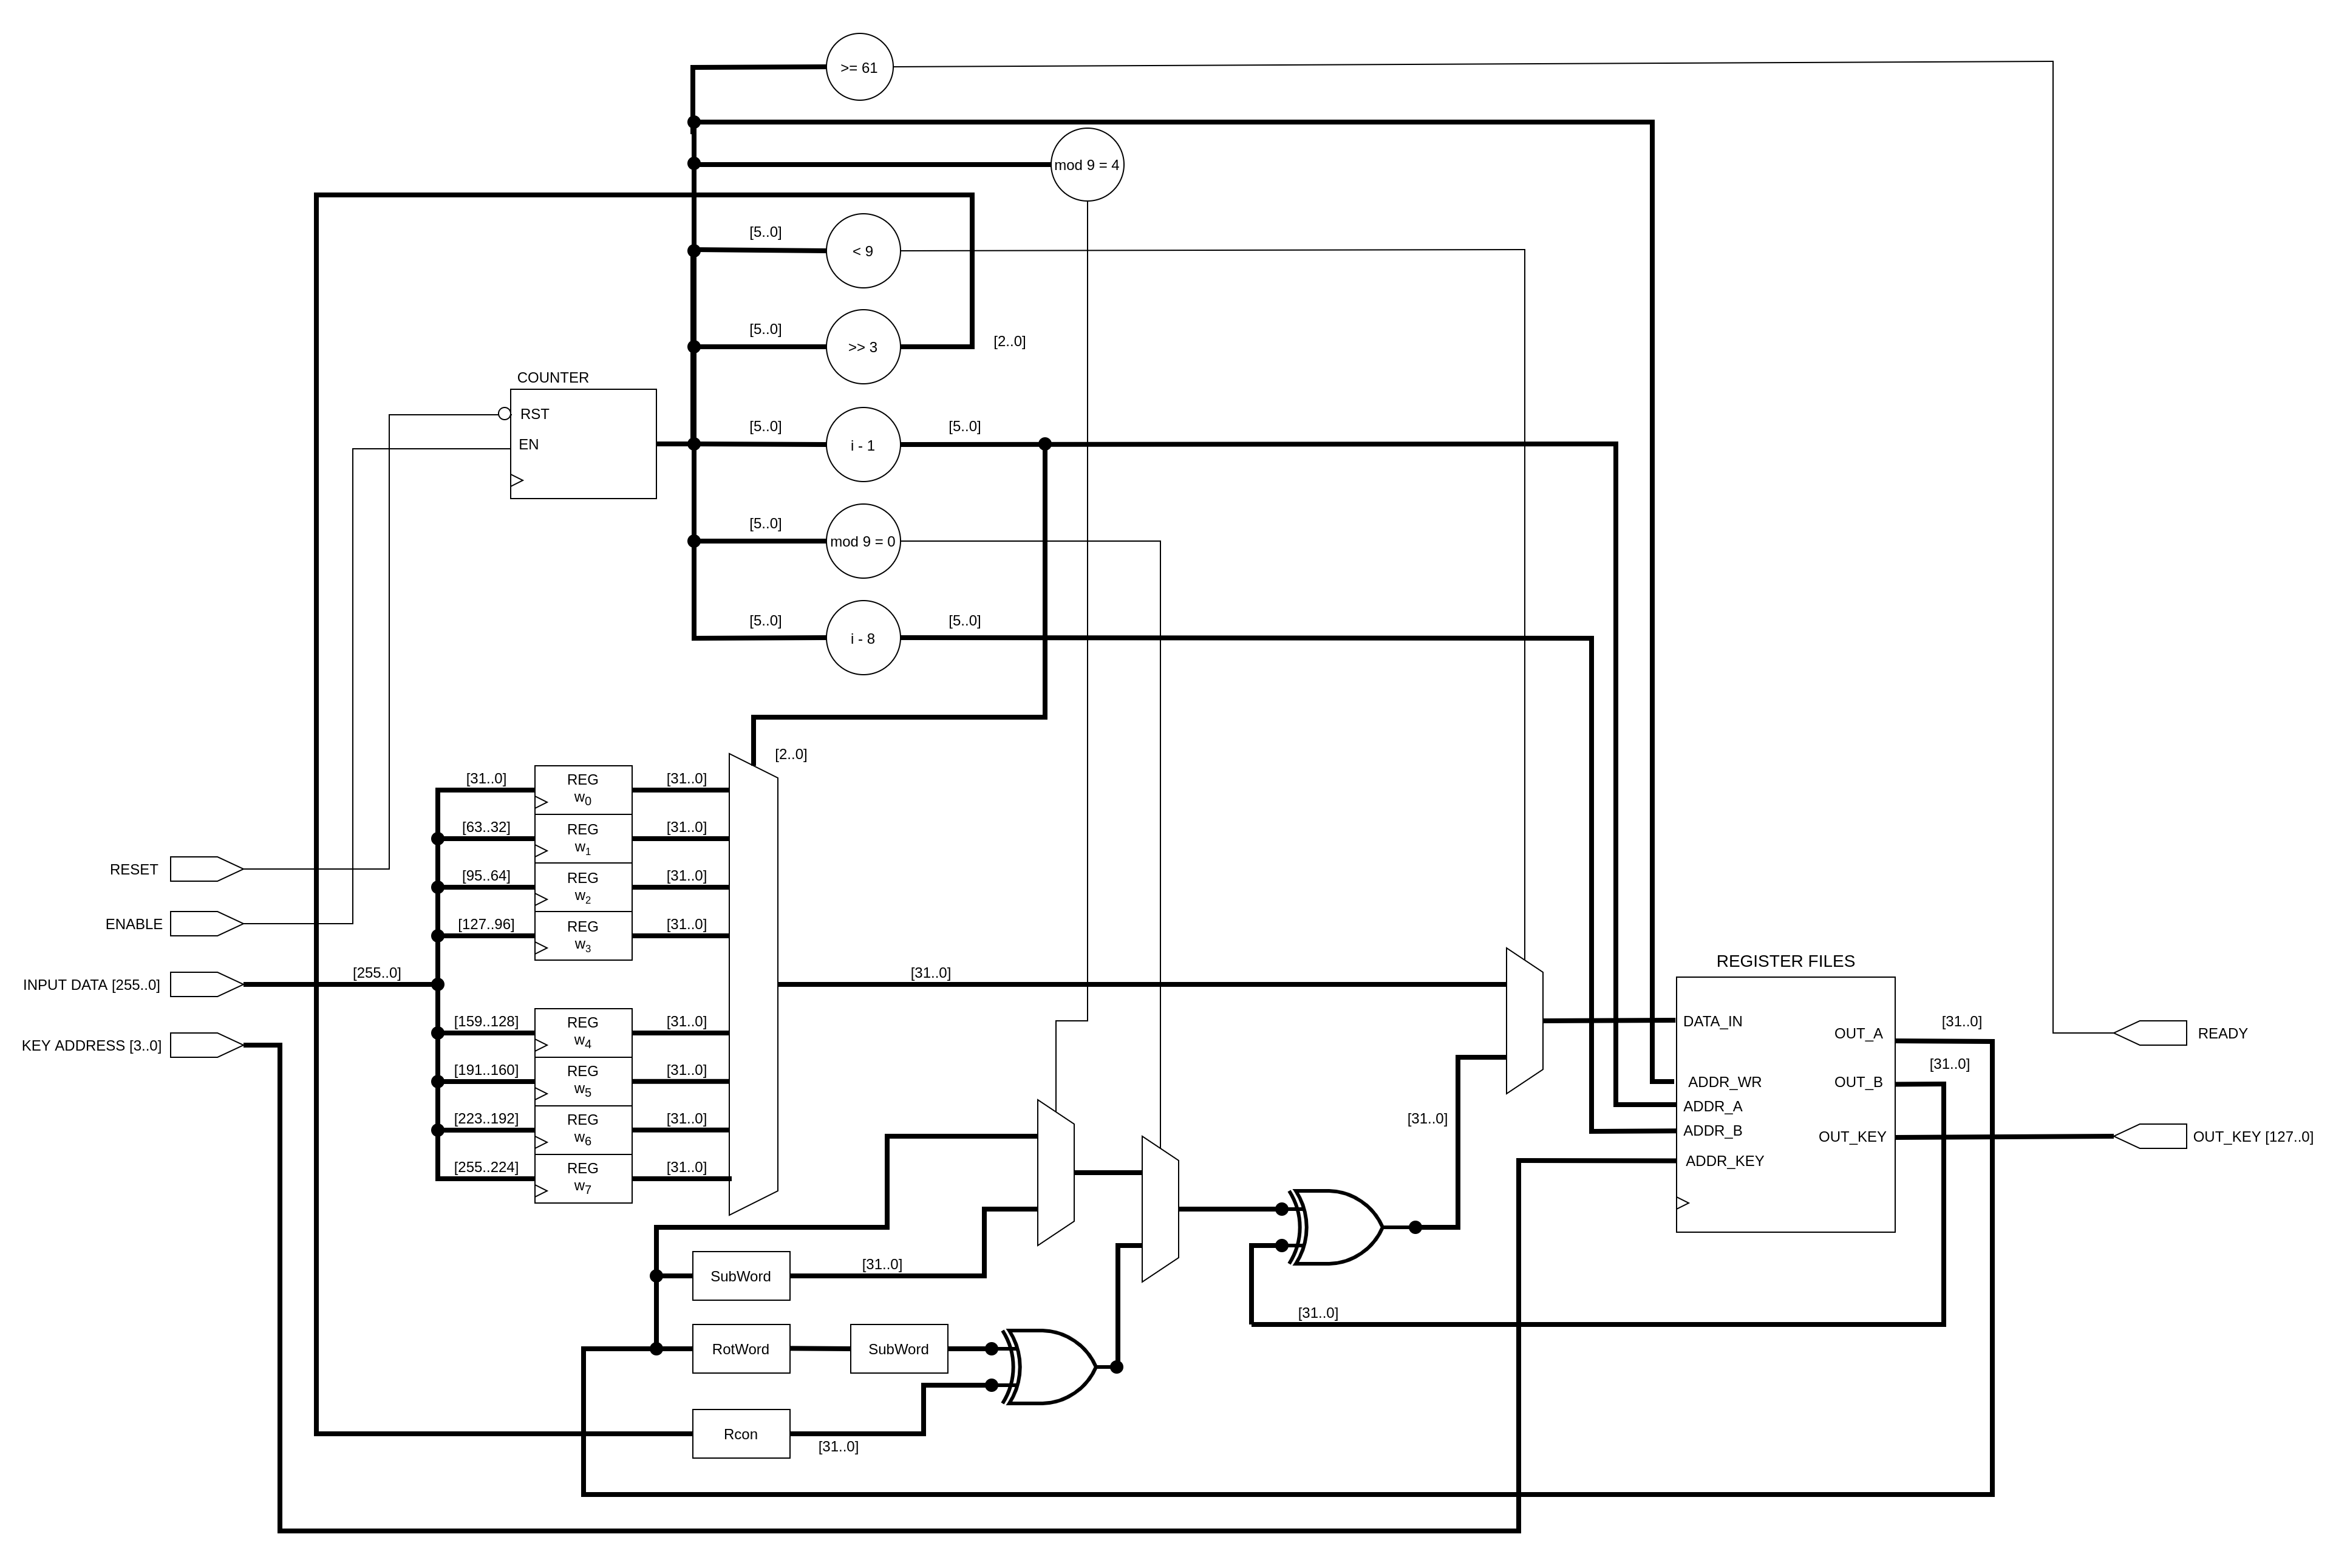
\includegraphics[width=\textwidth]{KeyExpansion.png}
            \caption{Diagram of Key Expansion.}
            \label{fig:KeyExpansion}
        \end{figure}

        \begin{multicols}{2}
        \section{IMPLEMENTATION}

            \subsection{Key Expansion}

            The design of the Key Expansion routine is shown in figure \ref{fig:KeyExpansion}. As in the design, the total of 15 round keys, including round key for the initial round, will be created firstbefore they could involve in the \textbf{\textit{Add Round Key}} function in the encryption and decryption process.
            
            This circuit will generate words that make up the Round Key one-by-one and store them in the \textit{Register File}. The \textit{Register File} has the total amount of 64 registers but only 60 of them are used because we only need to generate 60 words. The module \textit{Rcon} and \textit{SubWord} are implemented in the form of look-up tables (LUTs).

            In order for the circuit to work, the \textit{reset} signal must be pulled low (the \textit{reset} signal is active low) and then the \textit{enable} signal is pulled high. The cipher key can be passed through \textit{Input Data}. After reset, the counter's value will be set to zero and increased by 1 after each clock cycle. In the meantime, the inputted cipher key will be broken up into words, which are 32 bits each, and stored in eight registers from $w_{0}$ to $w_{7}$.
            
            In the next eight clock cycles each of the word will be saved into the \textit{Register File} sequentially from the address 1 to 8. After that, to generate the $i^{th}$ word, $(i-1)^{th}$ and $(i-Nk)^{th}$ words are required, which can be accessed through Register File's Out\_A \& Out\_B ports respectively, with the addresses are selected by $i-1$ \& $i-8$ blocks in the circuit.
            
            Depend on which word is generating, \textit{RotWord}, \textit{SubWord} can all be performed or just \textit{SubWord} is performed or neither of those. This is controlled by signals from \textit{mod 9 = 4} \& \textit{mod 9 = 0} blocks. Basically, the \textit{mod 9 = 4} block checks if a input number dividing by 9 has 4 as the remainder. If it is, the output will be pulled high and pulled low if it is not. Same thing with the \textit{mod 9 = 0} block but with 0 as the remainder. The design of \textit{mod 9 = 0} \& \textit{mod 9 = 4} are shown in figure \ref{fig:mod9eq0} \& figure \ref{fig:mod9eq4}, respectively.
            
            \noindent
            \begin{Figure}
                \centering
                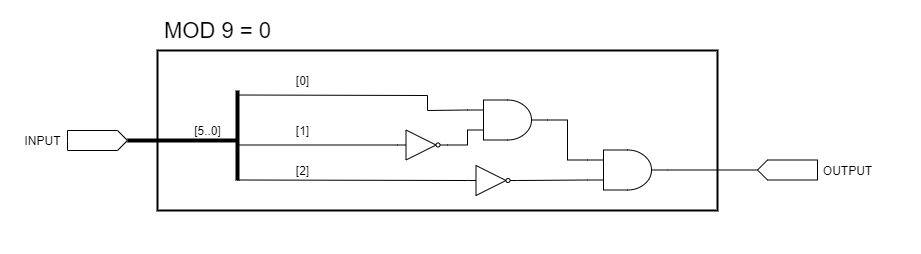
\includegraphics[width=\linewidth]{Mod9Eq0.png}
                \captionof{figure}{Circuit of \textit{mod 9 = 0} block}
                \label{fig:mod9eq0}
            \end{Figure}

            \noindent
            \begin{Figure}
                \centering
                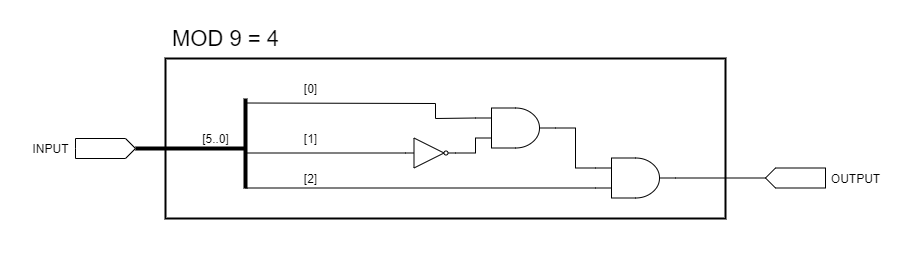
\includegraphics[width=\linewidth]{Mod9Eq4.png}
                \captionof{figure}{Circuit of \textit{mod 9 = 4} block}
                \label{fig:mod9eq4}
            \end{Figure}

            All the words will have been generated after sixty-one clock cycles. The counter will shut it self and the \textit{ready} signal is set indicating all round keys have been generated. After done generating and the \textit{ready} signal is set, round keys can be accessed by inputting the appropriate address through \textit{Key Address} input, which have the value range from 0 to 14.

            \subsection{Bytes Substitution}

            \noindent
            \begin{Figure}
                \centering
                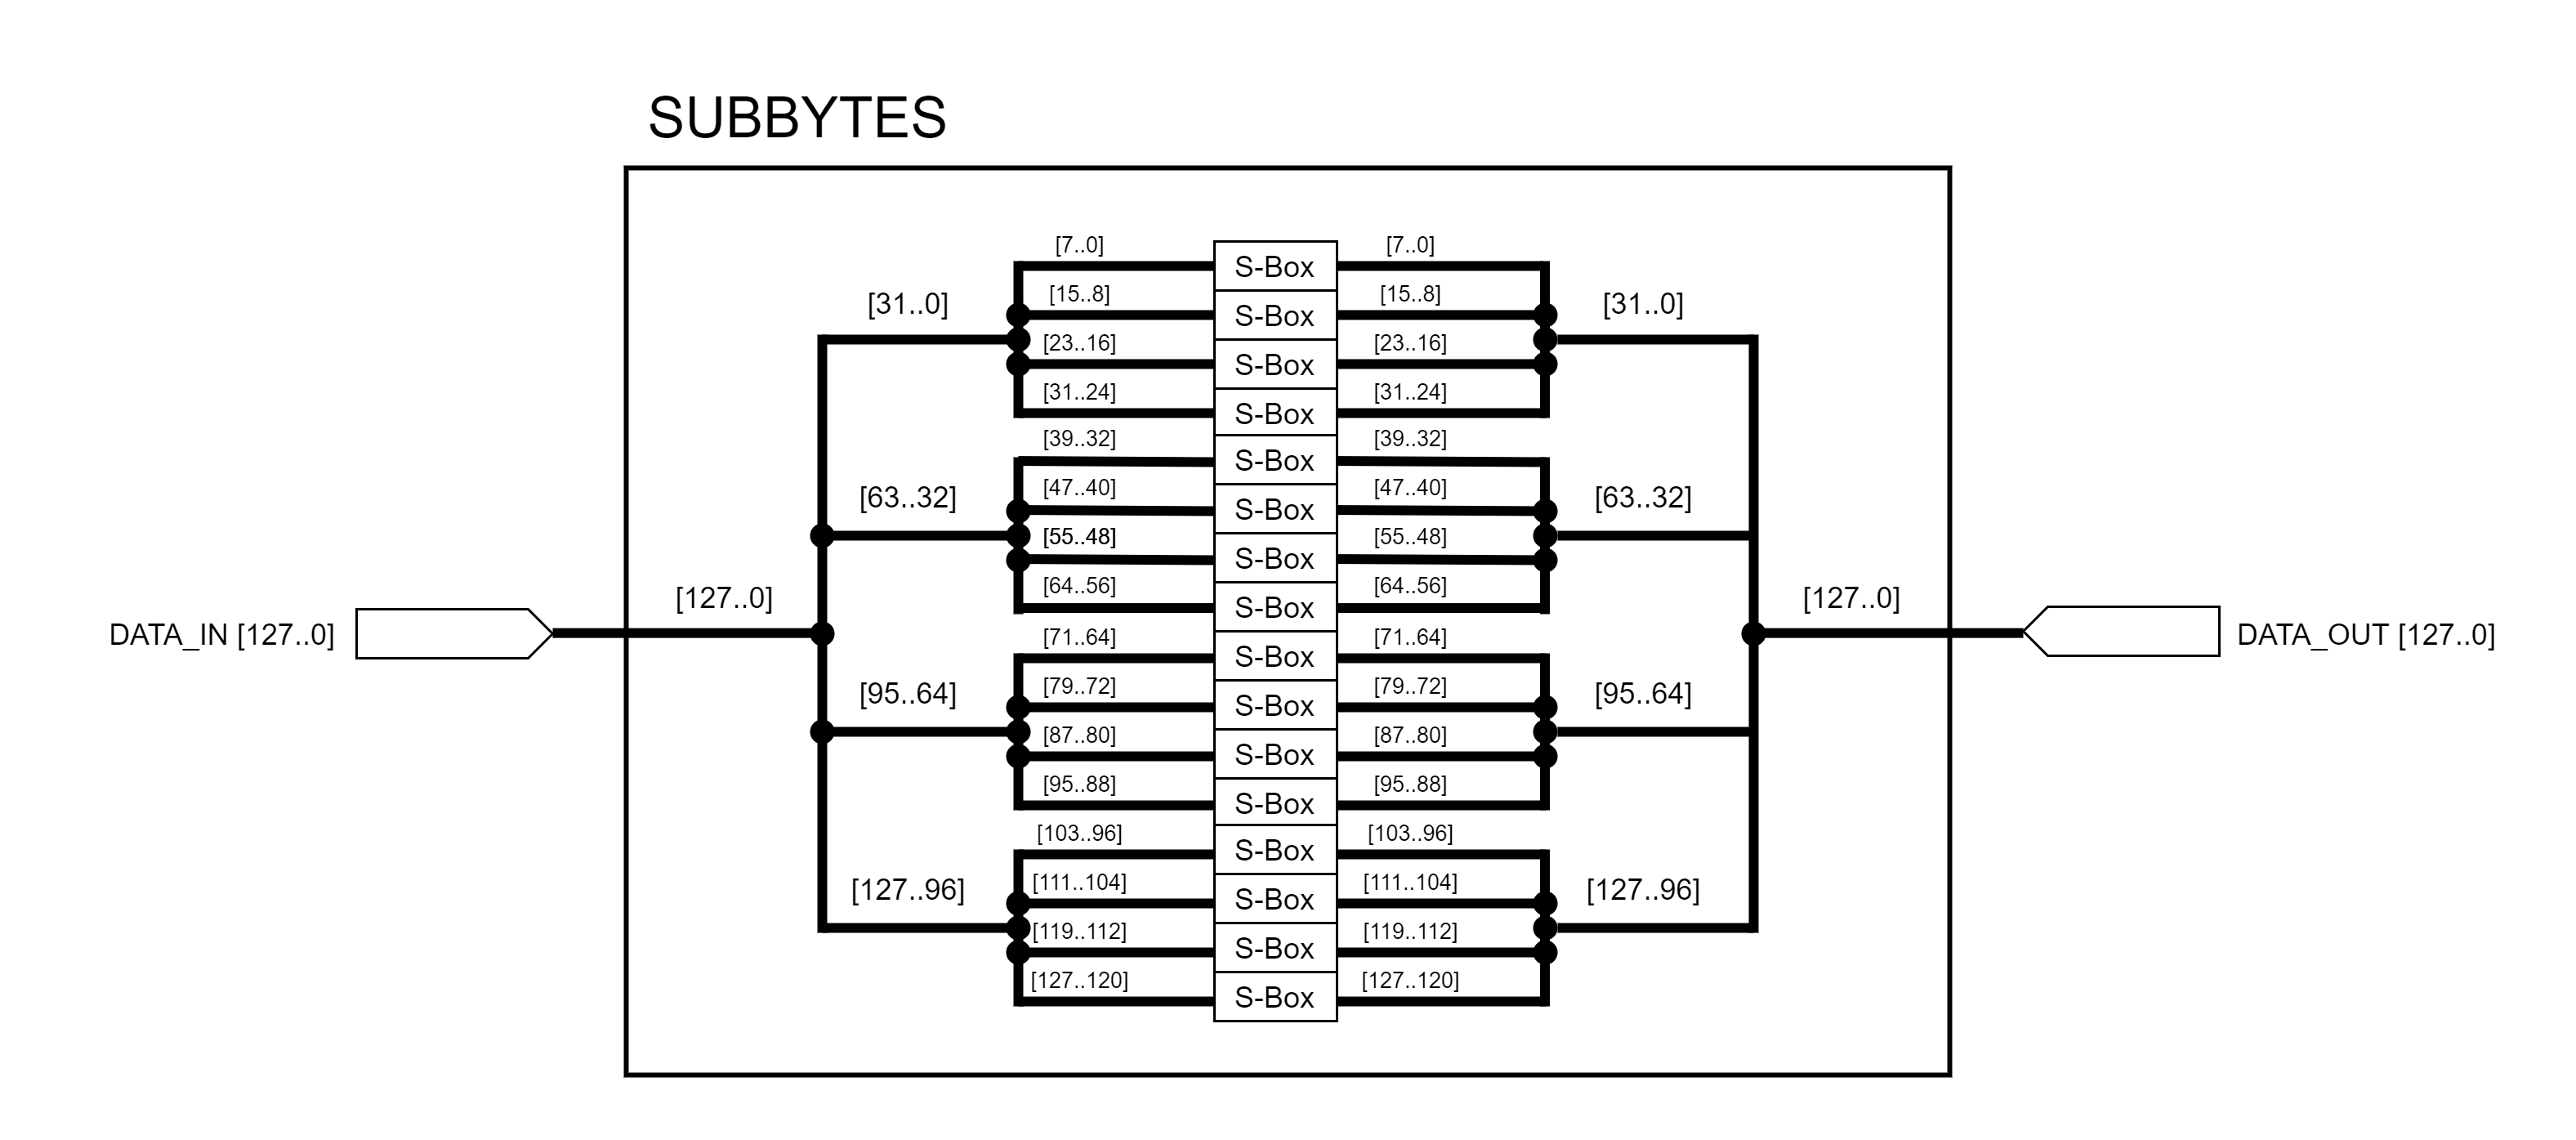
\includegraphics[width=\linewidth]{SubBytes.png}
                \captionof{figure}{SubBytes circuit diagram.}
                \label{fig:subbytes}
            \end{Figure}

            The design for \textit{SubBytes} block is shown in figure \ref{fig:subbytes}. The \textit{SBox} used in this circuit is implemented as LUT and is the same as \textit{SBox} from figure \ref{fig:SBox} and \textit{SubWord} in \textit{Key Expansion} routine.

            This ciruit takes 128-bit data and splits into words and then into individual bytes. Each byte will be fed into \textit{SBox} and the corresponding byte will be outputted. The outputted bytes will then be combined into words and eventually into 128-bit output data.

            \subsection{Shift Rows}

            \noindent
            \begin{Figure}
                \centering
                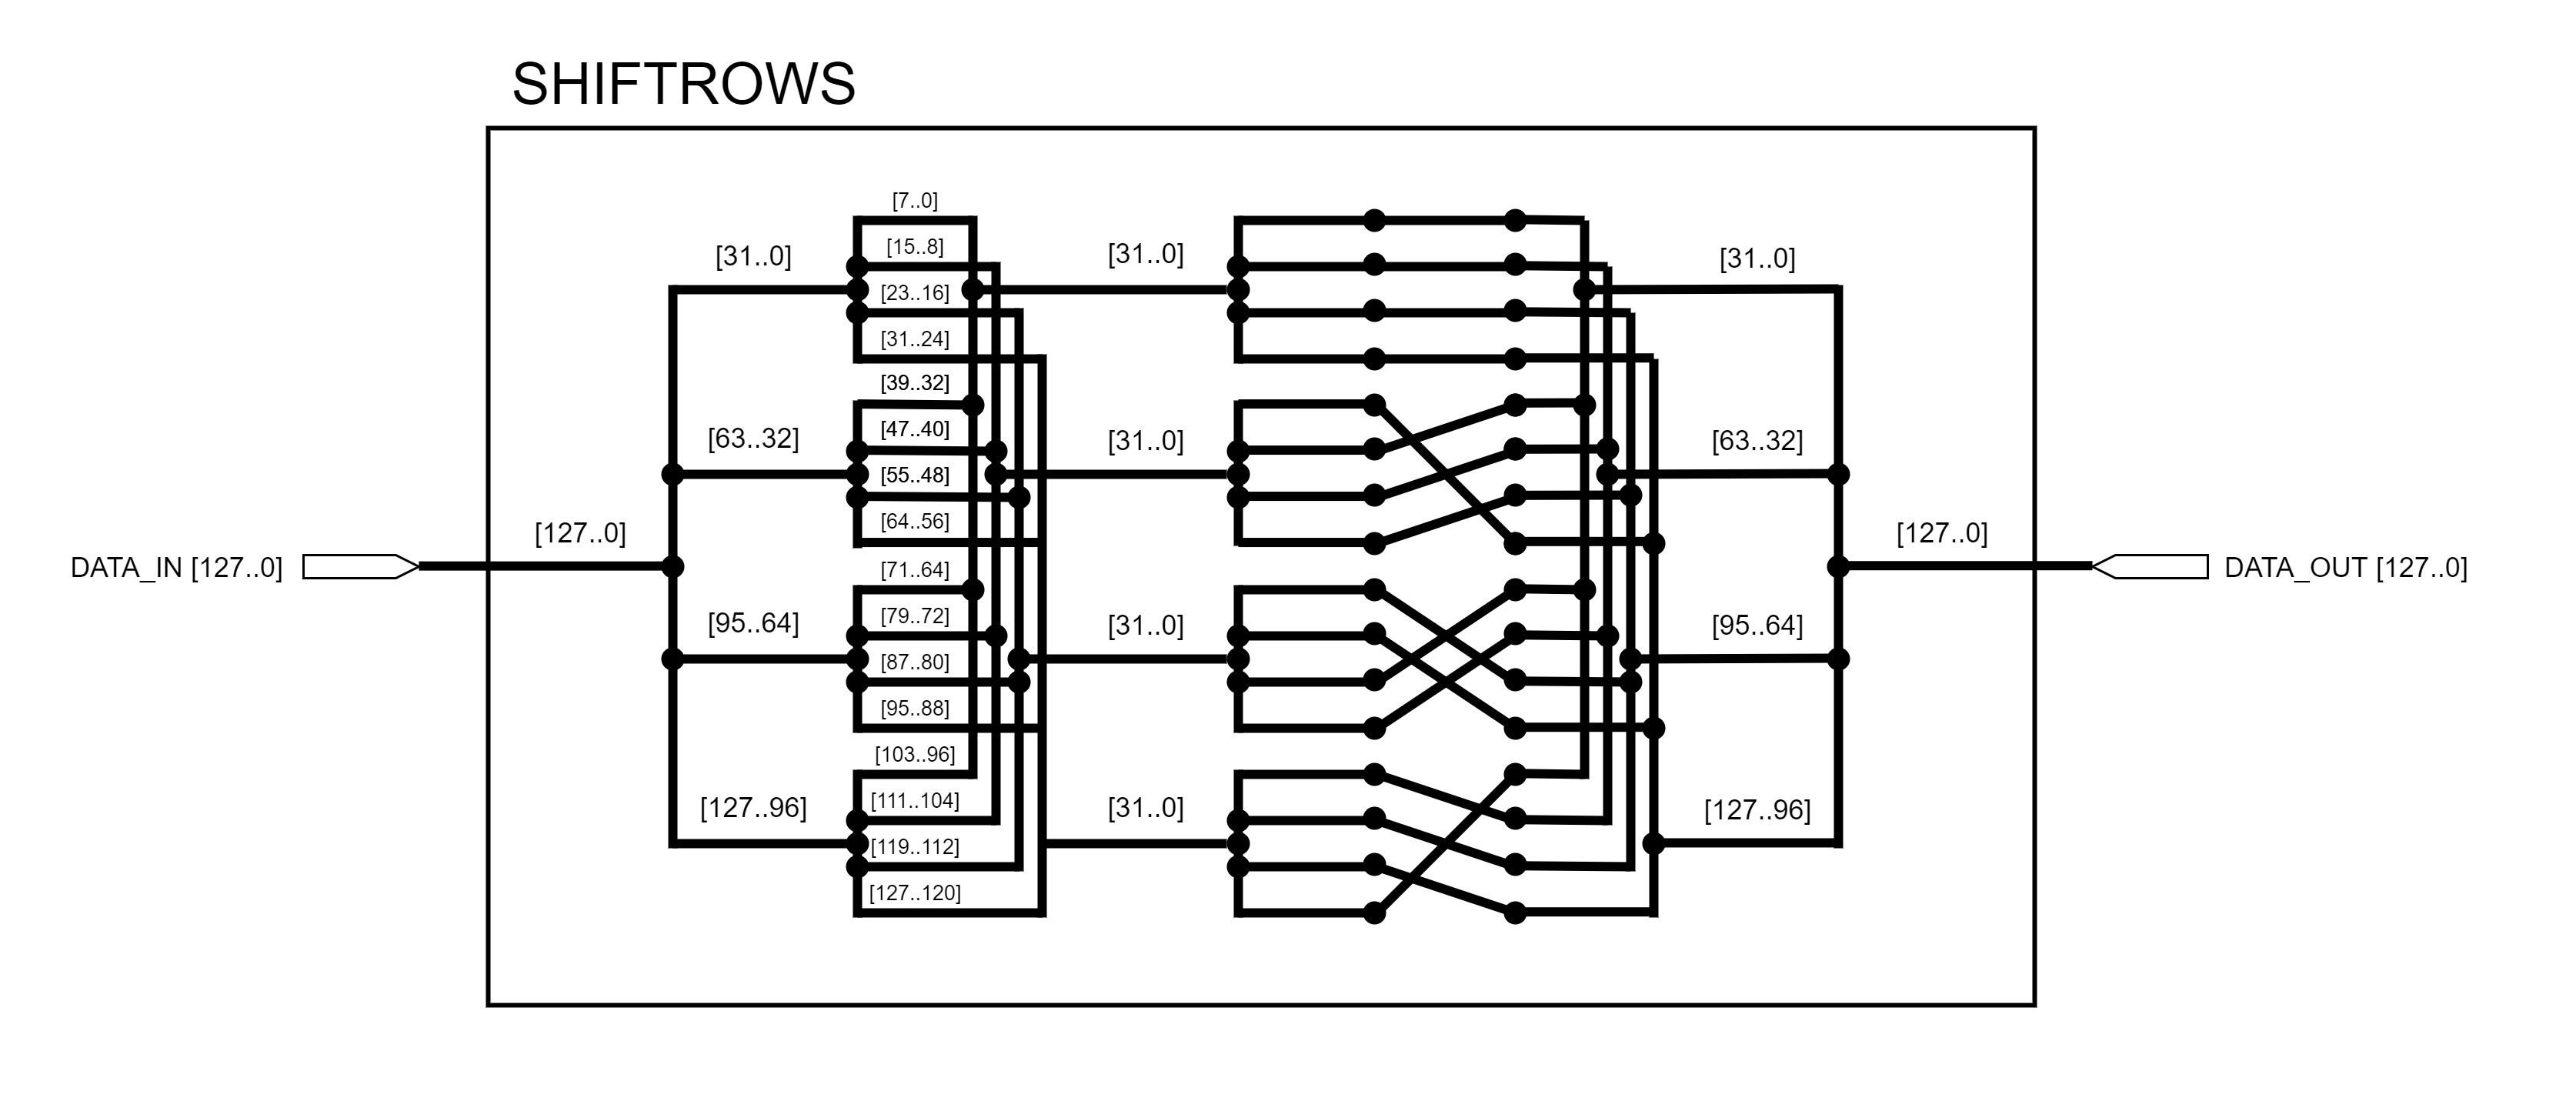
\includegraphics[width=\linewidth]{ShiftRows.png}
                \captionof{figure}{ShiftRows circuit diagram.}
                \label{fig:shiftrows}
            \end{Figure}

            The circuit diagram for \textit{ShiftRows} is shown in figure \ref{fig:shiftrows}. This circuit takes 128-bit data in, perform shifting and output 128-bit data.

            The inputted data will first be split into 32-bit words, note that each word corresponds to a column in the \textit{State}. The first row is formed by taking the first byte in each word, and the second byte in each word for the second row and so on for the third and fourth rows. After dividing the input into rows, the shifting operation is done by wiring each row with the corresponding offsets which discussed in section \ref{sec:shift-rows-intro}.

            Finally, all the rows will be split and combined into correct columns and rows format of the \textit{State}.

            \subsection{Mix Columns}

            \noindent
            \begin{Figure}
                \centering
                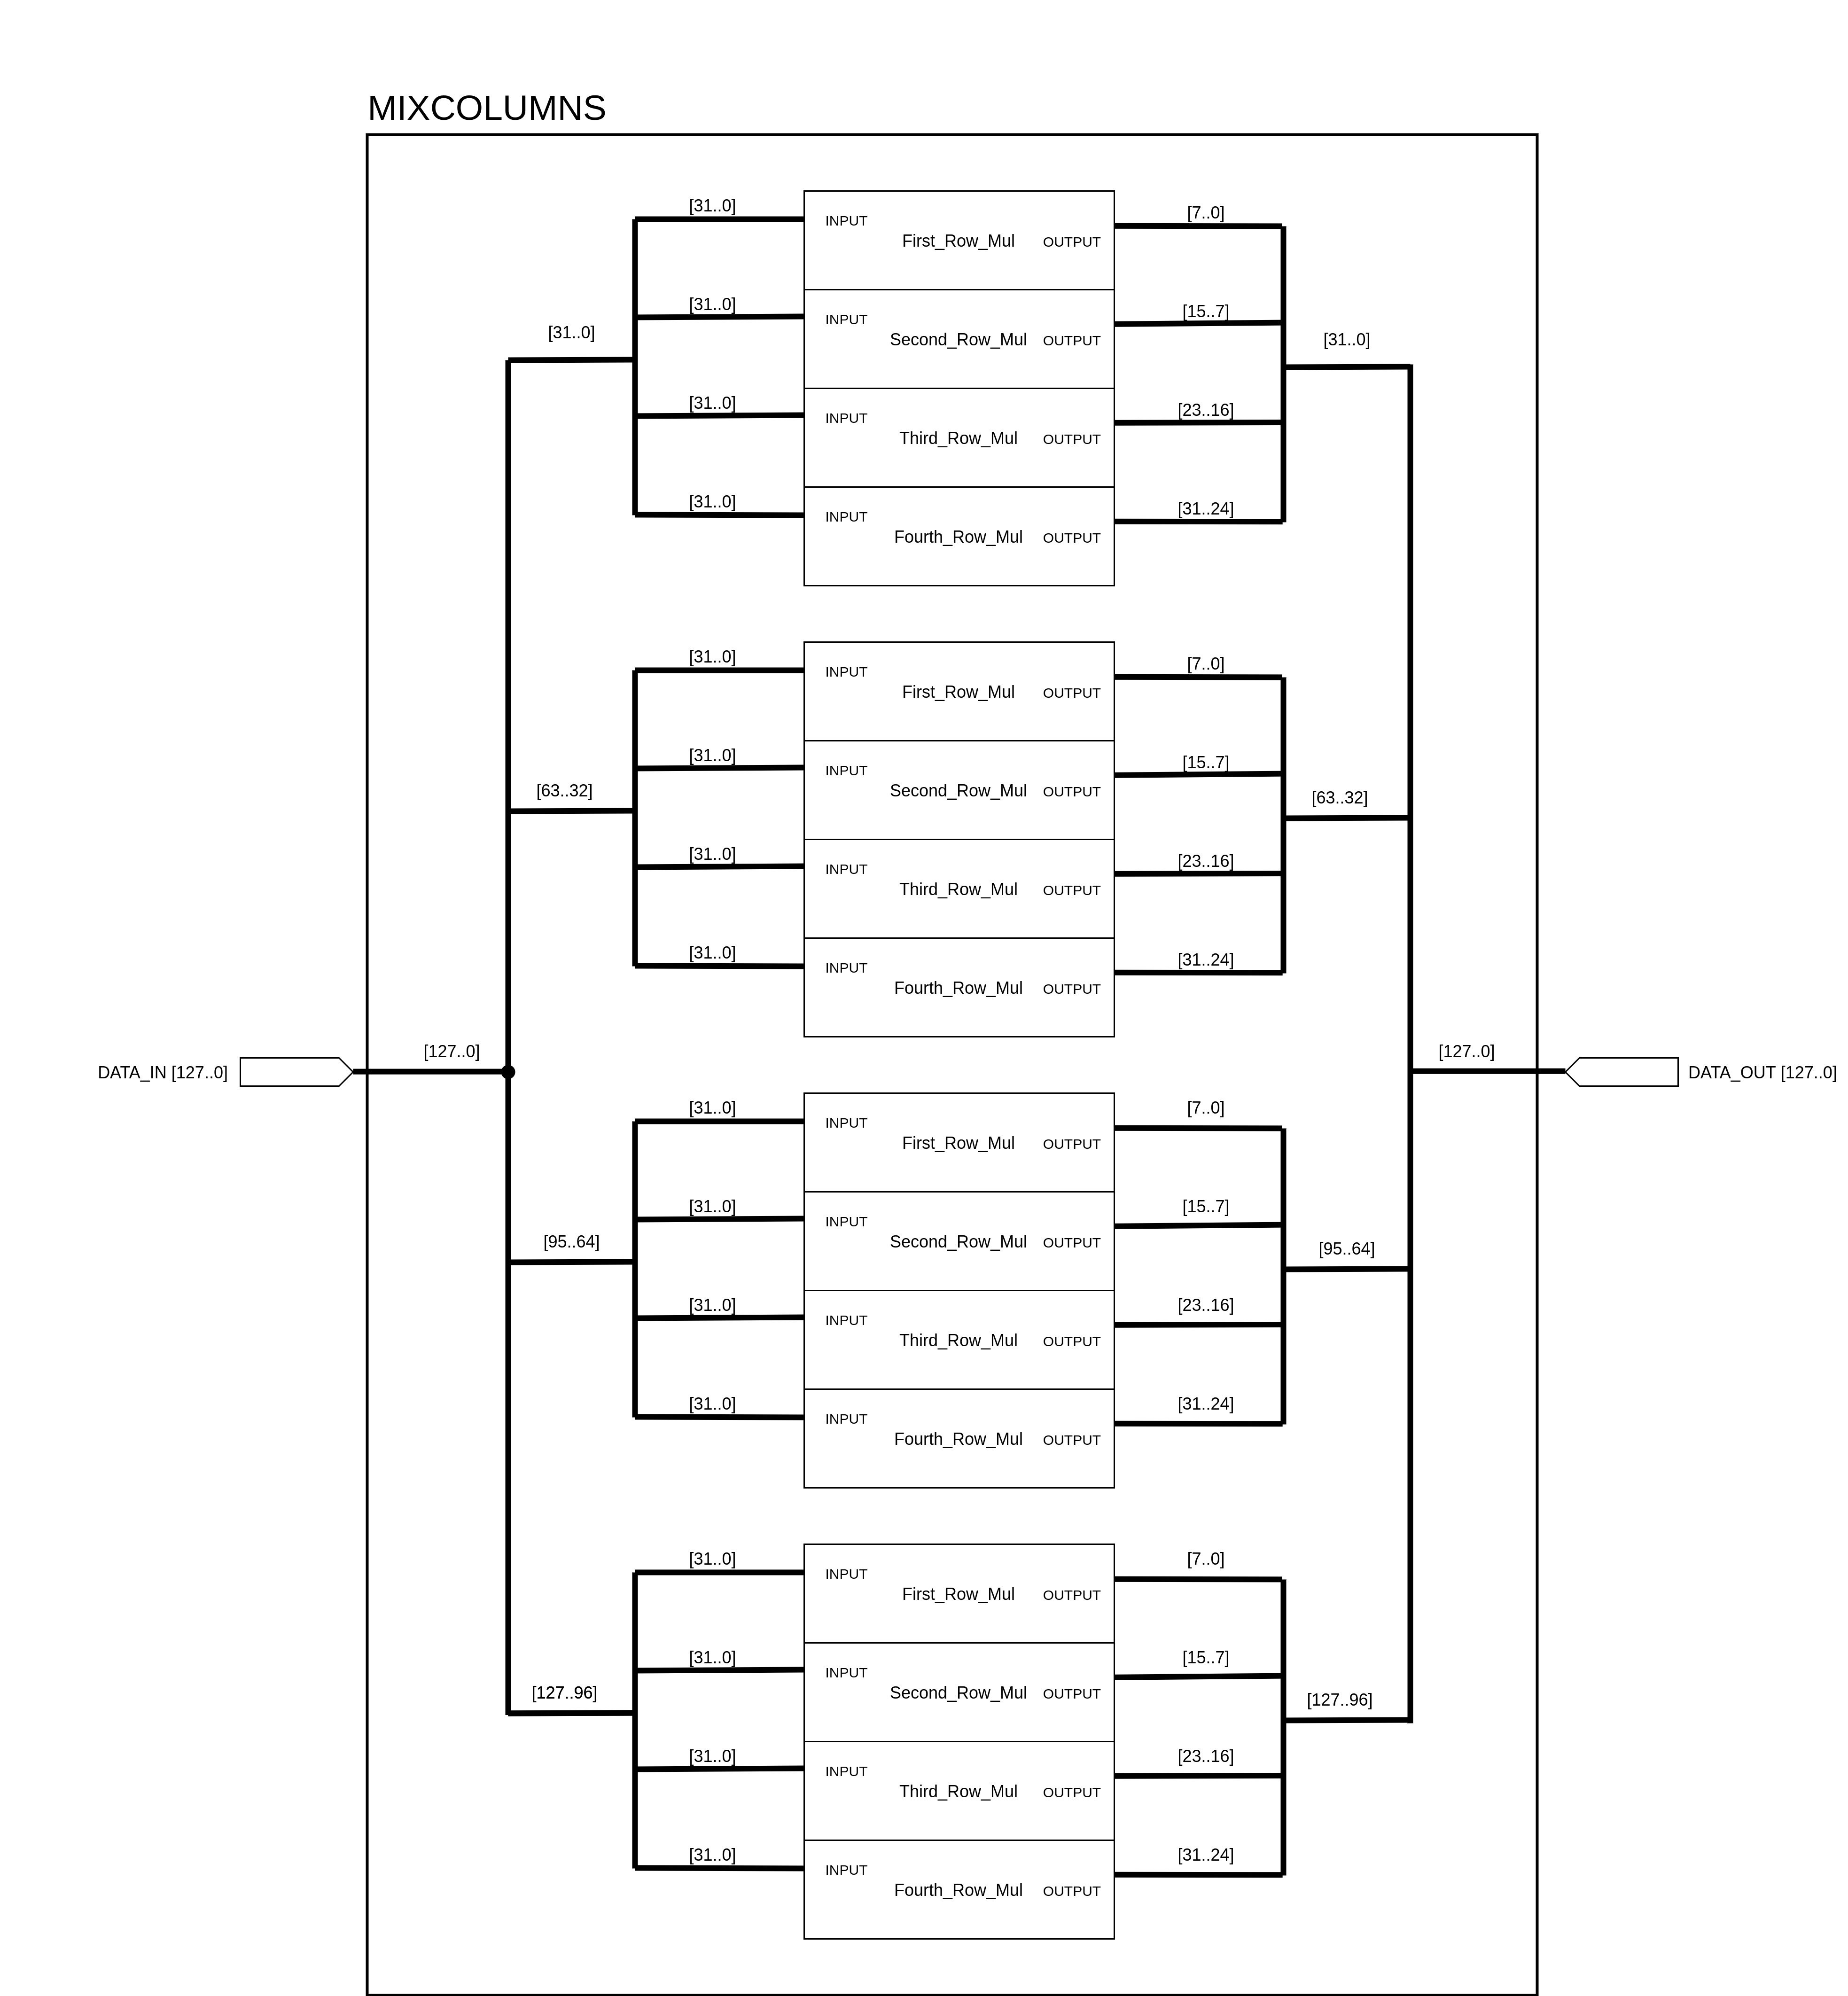
\includegraphics[width=\linewidth]{MixColumns.png}
                \captionof{figure}{MixColumns circuit diagram.}
                \label{fig:mixcolumns}
            \end{Figure}

            Text here.

            \noindent
            \begin{Figure}
                \centering
                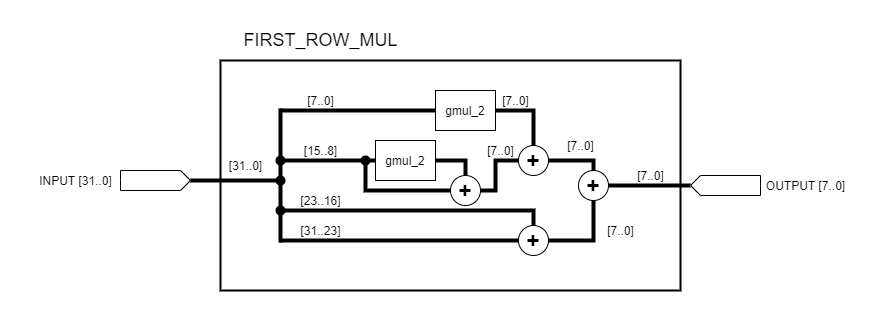
\includegraphics[width=\linewidth]{First_Row_Mul.png}
                \captionof{figure}{First\_Col\_Mul.}
                \label{fig:first-col-mul}
            \end{Figure}

            \noindent
            \begin{Figure}
                \centering
                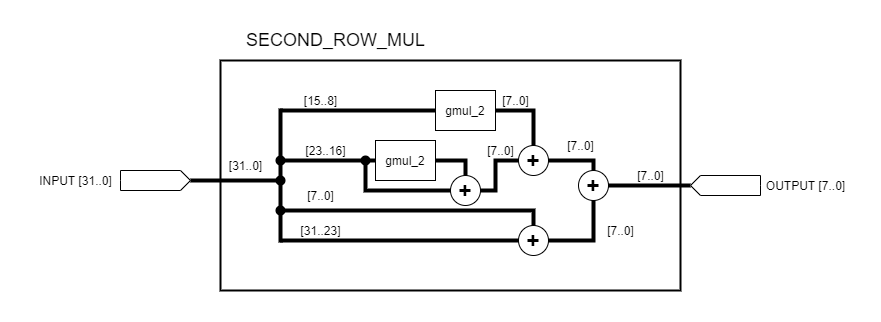
\includegraphics[width=\linewidth]{Second_Row_Mul.png}
                \captionof{figure}{Second\_Row\_Mul.}
                \label{fig:second-row-mul}
            \end{Figure}

            \noindent
            \begin{Figure}
                \centering
                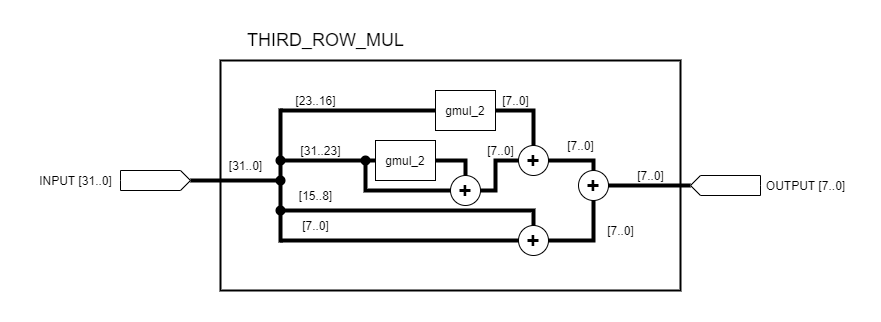
\includegraphics[width=\linewidth]{Third_Row_Mul.png}
                \captionof{figure}{Third\_Row\_Mul.}
                \label{fig:third-row-mul}
            \end{Figure}

            \noindent
            \begin{Figure}
                \centering
                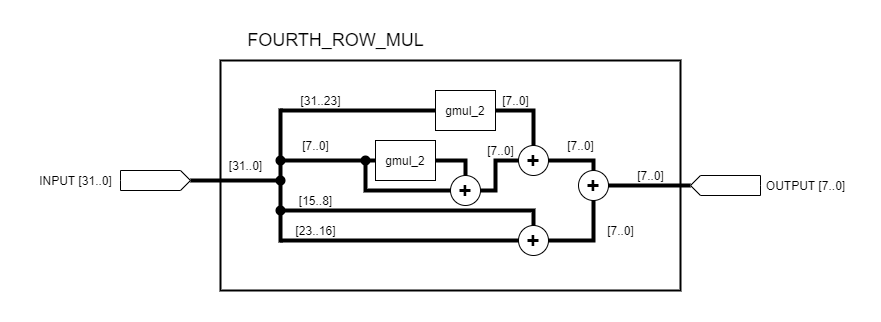
\includegraphics[width=\linewidth]{Fourth_Row_Mul.png}
                \captionof{figure}{Fourth\_Row\_Mul.}
                \label{fig:fourth-row-mul}
            \end{Figure}

            \noindent
            \begin{Figure}
                \centering
                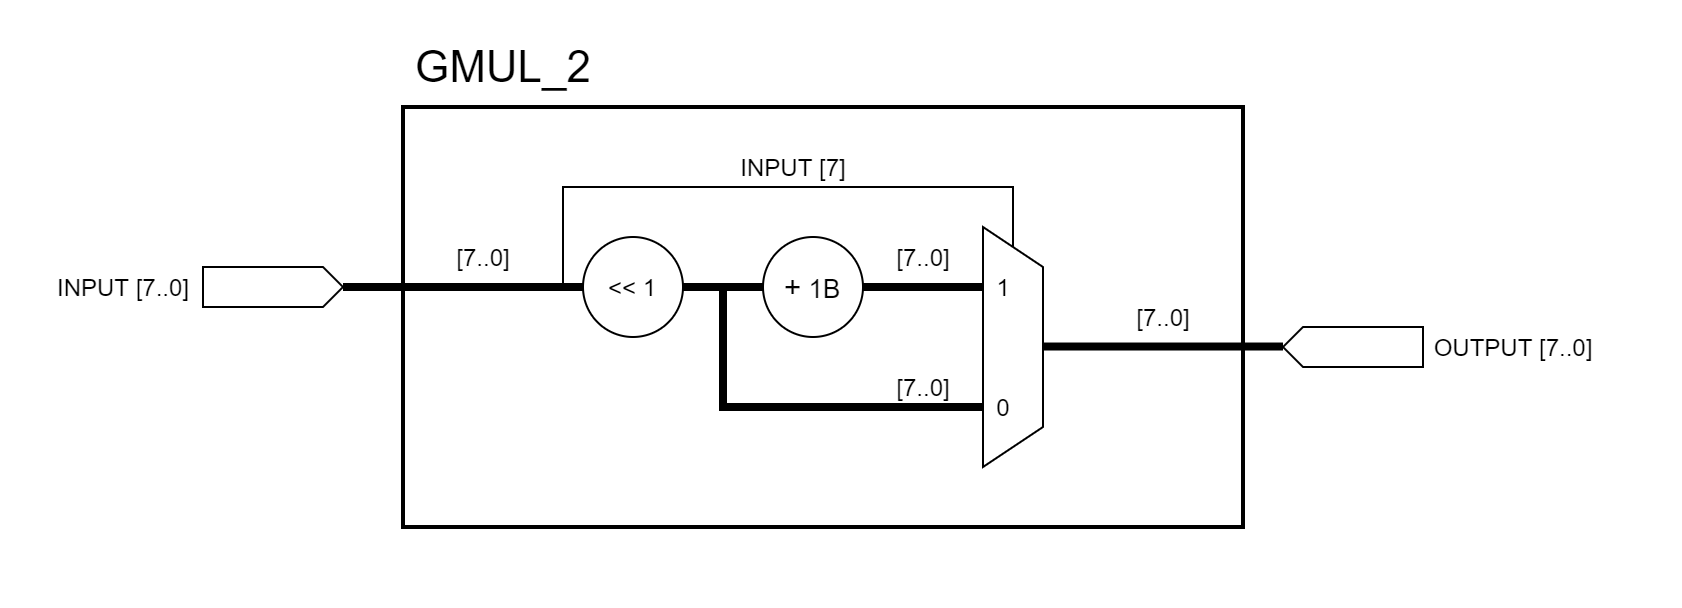
\includegraphics[width=\linewidth]{gmul_2.png}
                \captionof{figure}{gmul\_2.}
                \label{fig:gmul-2}
            \end{Figure}

            \subsection{Add Round Keys}

            Text here.

        \section{RESULTS}

        (N/A)

        \section{CONCLUSION}

        (N/A)

        %%%%%%%%%%%%%%%%%%%%%%%%%%
        % REFERENCE SECTION HERE %
        %%%%%%%%%%%%%%%%%%%%%%%%%%
        \begin{thebibliography}{3}
            \bibitem{AES}
            Federal Information Processing Standard (FIPS) 197.
            \textit{Advanced Encryption Standard (AES)}
            26 November 2001.

            \bibitem{sam-key-expansion}
            Sam Trenholme.
            \textit{Rijndael's key schedule.\\https://samiam.org/key-schedule.html}.

            \bibitem{sam-mix-columns}
            Sam Trenholme.
            \textit{Rijndael's mix column stage.\\https://samiam.org/mix-column.html}.

            \bibitem{sam-galois-field}
            Sam Trenholme.
            \textit{AES' Galois field.\\https://samiam.org/galois.html}.

            \bibitem{sam-s-box}
            Sam Trenholme.
            \textit{Rijndael's S-Box.\\https://samiam.org/s-box.html}.

            \bibitem{understand_mixcol}
            Kit Choy Xintong.
            \textit{Understanding AES Mix-Columns Transformation Calculation}.
        \end{thebibliography}

    \end{multicols}

\end{document}
